%===================================== CHAP 5 =================================

\chapter{Implementation}\label{ch5:implementation}

To be able to answer the research questions using the methods described in the previous chapter, a prototype needed to be developed. This chapter covers the implementation and architecture of that prototype, named Utsida, and introduces its different parts, components, design and usability choices, and test environment.

\section{System Overview}

Utsida contains two sub-systems, where the first part is a web application, and the second part is a case-based reasoning recommender system (CBR-RS). Each part primarily focuses on one of the research questions. The web application is designed to increase the motivation (RQ1), while the CBR-RS is designed to find out how suitable CBR is to give recommendations on exchange universities and courses (RQ2). The recommendations made by the CBR-RS could also affect the motivation (RQ1). Utsida was chosen as the name of the system due to being a counter opposite to NTNU's central system \emph{Innsida}, and the meaning of the word \emph{inside}. Utsida gives a relation to something on the outside, in this case going on an exchange program. The design and implementation of Utsida was based on the system requirements (sec. \ref{sec:requirements}) identified in the preliminary research.

As illustrated by Figure \ref{fig:system_overview}, the web application part communicates with the CBR-RS part. Recommendation queries are sent from the web application by a user and received by the CBR-RS through its Representational State Transfer (REST) Application Programming Interface (API). These queries are in turn matched against the entire case-base in the CBR-RS. Finally, all the cases are given a similarity score based on the user query and the most similar cases are returned to the web application. The user can then select a specific case from the several recommendations shown in the web application.

\begin{figure}[H]
    \centering
    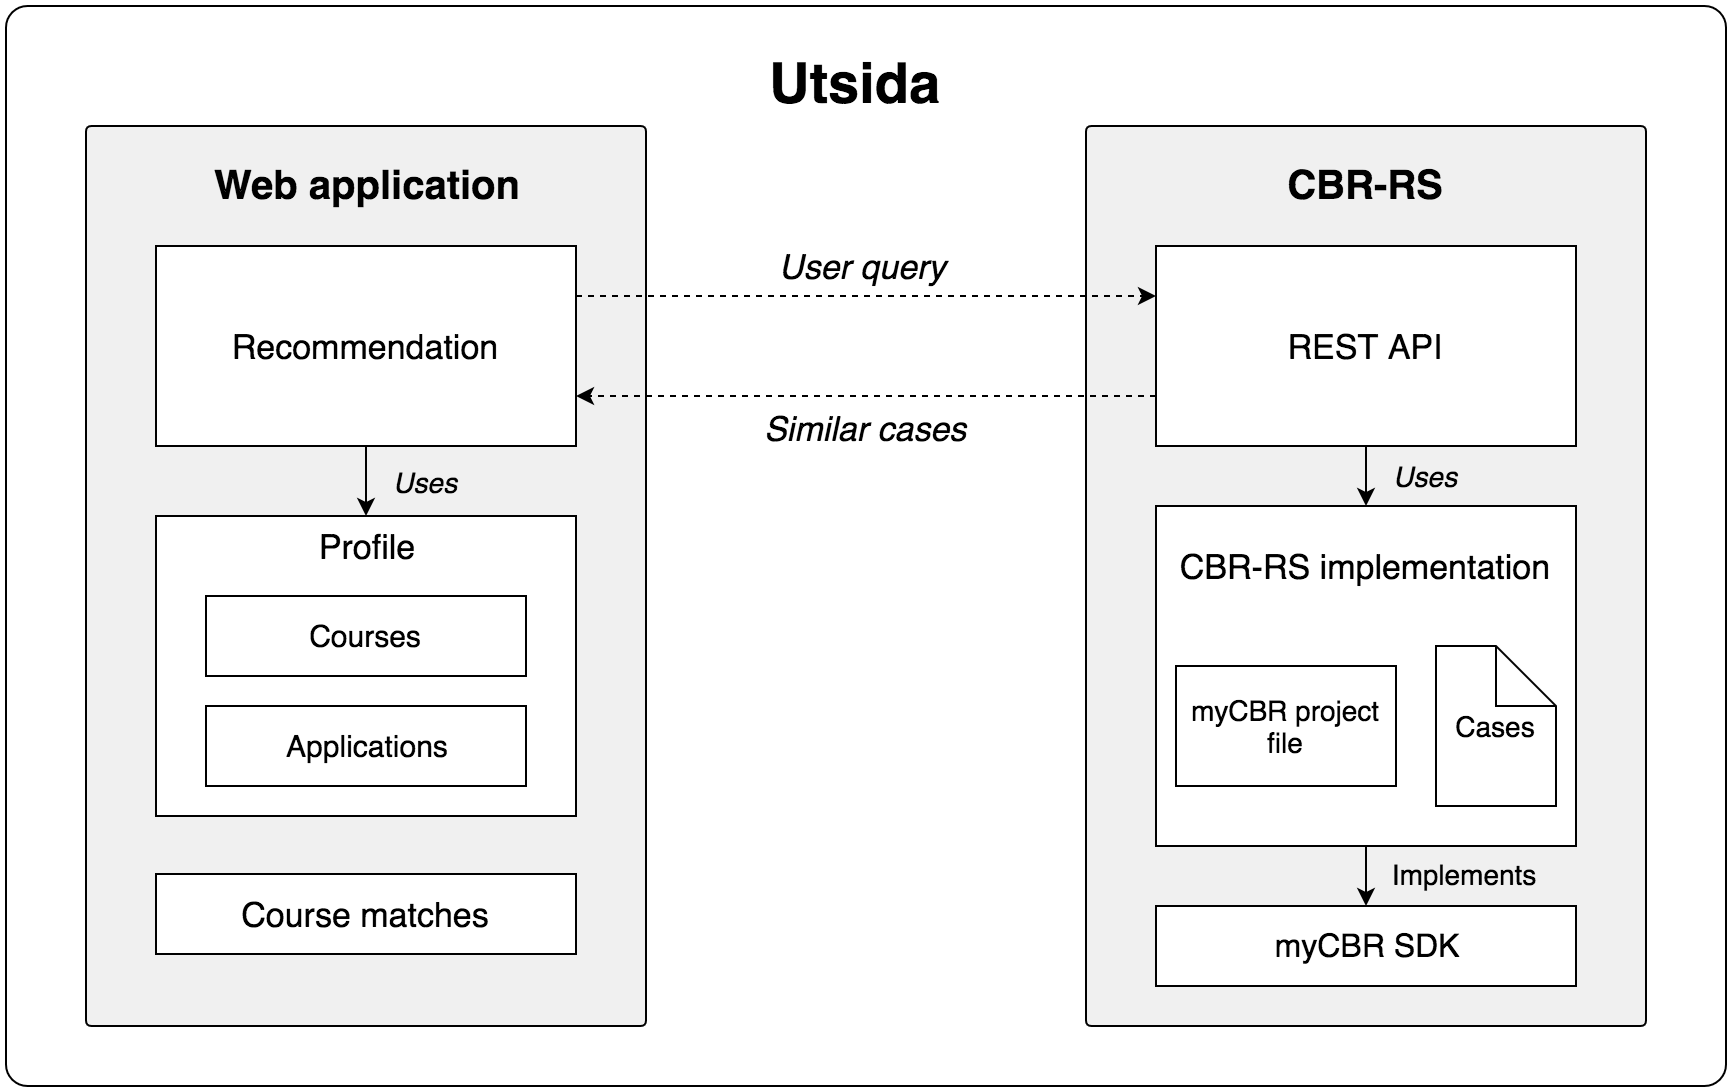
\includegraphics[width=1\textwidth]{fig/system_overview.png}
    \caption{Architectural overview of Utsida}
    \label{fig:system_overview}
\end{figure}

\section{Data and Information}

Utsida requires up to date organizational data about NTNU. This includes all the courses, faculties, and departments at NTNU. The required organizational data was gathered with IDI's organizational API\footnote{http://www.ime.ntnu.no/api/}. This API was, however, recently discontinued, so to update this data after 2016, a new data source would have to be found. Furthermore, the course matches component (sec. \ref{sec_course_matches}) in the web application relies on information on previously approved course matches\footnote{Sets of courses where one or more courses from another university are approved by advisers as a replacement for a course at NTNU}. To avoid a cold start, some approved course matches from IDI were parsed and used in the component. The most critical data, however, was the data used to create cases for the CBR-RS, namely the \textit{experience reports}. All data used in Utsida was analyzed according to the six primary dimensions for data quality assessment \cite{askham2013six} to gain awareness of the possible limitations before deciding on Utsida's database models.

\subsection{The Experience Reports}\label{sec:experience_reports}

Most students who go on an exchange program from NTNU have to write obligatory reports about their exchange experience to the OIR. These reports are available to the public, and are written in the period between 1999 and 2016. Because the reports include a large amount of information on exchange experiences, they were used as the data foundation for the cases. Typically, the case-base in a CBR-RS start off with a low amount of cases and gradually expand as new cases are retained. In this project, however, it was essential to have an initially large number of cases. Therefore, all of the current public experience reports were parsed and used as cases in the CBR-RS' case-base. 

\subsection{Parsing the Experience Reports}\label{sec:parsing_experience_reports}

The experience reports are essentially large text files in Hypertext Markup Language (HTML) format. To be able to use them in the CBR-RS, all the useful information in the files had to be extracted and parsed to cases in a CSV file, which is the file format used for case-bases in myCBR. This was done with a custom script written in the Python programming language. In short, all available experience reports were first downloaded as HTML files and stored in a directory. Next, the script looped through all the HTML files, read the internal data, and finally stored all the chosen data in a CSV file. This way, each row in the CSV file would correspond to one case with the attributes given by Table \ref{tab:case_representation2}. This process resulted in a CSV file with 8702 cases which formed the case-base used in the CBR-RS.

A large part of the text fields in the experience reports were free text, which means that the format of each field was decided by the author and did follow any standard. The parsing script, therefore, had to use specific methods to parse each attribute to the correct format. Two methods were primarily used to parse the data; data dictionary look-ups and approximate string matching, also called fuzzy searching. Edge cases that were not detected by these techniques were solved with basic string operations. In the end, most of the data in the experience reports was transformed into usable data in the CBR-RS. It was, however, not possible to ensure that all of the data in the experience reports were parsed to a correct format while still keeping its original meaning.

Fuzzy Searching is an algorithm used to determine the similarity between two textual inputs. It calculates a similarity score between two textual inputs by recognizing patterns and similarities in the two inputs. By using fuzzy searching in the parser script, the data in the experience reports could be mapped against a predefined set of attributes, and return the attribute with the highest similarity. For example, the department field in the experience reports had a significant variation of abbreviations and ways of spelling. By creating a dictionary with all departments and faculties, fuzzy searching could be used to find the department in the dictionary with the highest similarity to the department in the experience report. This is illustrated in Figure \ref{fig:fuzzy_searching}. This method was also used on the university field to avoid creating multiple instances in the database. Several more Python dictionaries were configured to be able to map the necessary data in the experience reports to a correct format. These includes dictionaries for countries, continents, languages, universities, departments, and faculties.

\begin{figure}[h]
    \centering
    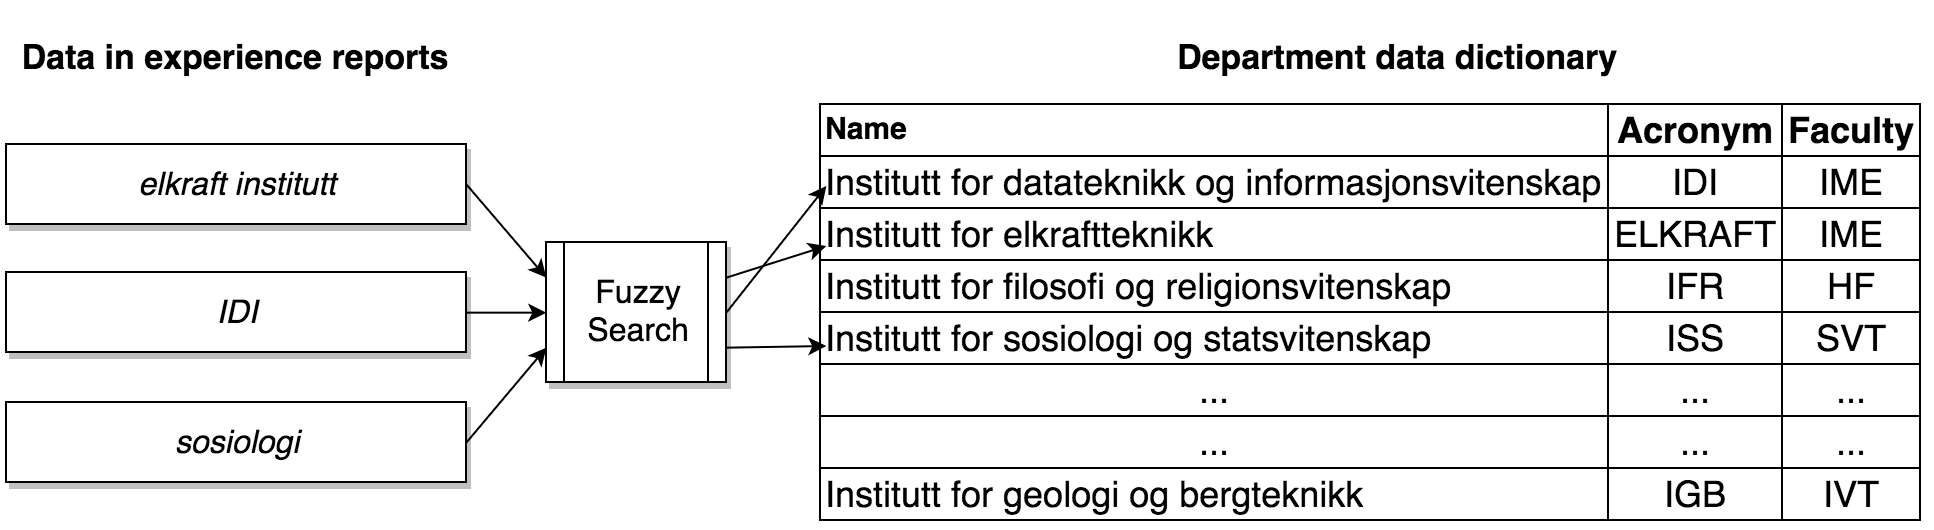
\includegraphics[width=1.0\textwidth]{fig/fuzzy_search2.png}
    \caption[Fuzzy searching]{How fuzzy searching is used to convert fields in the experience reports to a standard format defined in a dictionary.}
    \label{fig:fuzzy_searching}
\end{figure}

\FloatBarrier

\section{The Web Application}

This section presents the different components of the web application, the tools and frameworks used, and reasoning for design and usability choices.

\subsection{Components}

The web application part of Utsida is divided into three main components, as Figure \ref{fig:system_overview} depicts: \emph{Recommendations, Profile} and \emph{Course matches}. The aim of the components as a whole is to answer RQ1 and increase the motivation of students to go on an exchange program. Each component targets one or several of the requirements of Utsida, listed in Table \ref{tab:feature_list} The requirements are referenced in a REQ.\# format, with \# as the requirement number. REQ.5 is handled by the web application home page and not by any component.

\subsubsection{Recommendation}

The recommendation component target REQ.1. This component handles all the communication with the CBR-RS part; Queries made by users are sent in the JavaScript Object Notation (JSON) format to the CBR-RS through Hypertext Transfer Protocol (HTTP) requests, which returns all of its cases and their respective similarity score, also in JSON format. In this component, a user can select their preferences and requirements for an exchange program. The user is then presented with a list of the best suiting universities for their query (Fig. \ref{fig:web_results_1}). The universities in the list can each be selected to show the best matching experiences for that university (Fig. \ref{fig:web_results_2}). Each experience contains a list of courses taken and serves as a recommendation.

\subsubsection{Course Matches}\label{sec_course_matches}

The course matches component target REQ.2, and its purpose is to display all approved course matches stored in the web application. The component filters course matches by which university they are approved for, and supports adding, deleting, commenting and editing of course matches by student advisers. For a student, this component serves as a resource where they can: find replacements for their courses at NTNU, get information about the courses and the approval of them, and save the course match to their profile.

\subsubsection{Profile}

The profile component handles all profile functionality, such as authentication, and contains the required personal information about each student. One especially important information is the user's department, which is stored in the profile and used by the web application in a recommendation query. The component has two sub-components: Courses and Applications.

\paragraph{Courses} 
is a sub-component of the profile component and targets REQ.3. It contains functionalities which enable a student to organize their application process. This includes storing courses at home, courses abroad and course matches. From the course page, shown in Figure \ref{fig:web_courses}, students can also manually match abroad- and home courses to create new course matches for their applications. This component replaces a large part of the course match approval process and is essential for the digitalization of the process.

\paragraph{Applications} 
is another sub-component of the profile component and targets REQ.4. It stores user submitted applications that contains the course matches a user wants to get approved. It also maintains the functionality needed to create applications. For students and student advisers, the application component serves as a digital version of the current paper-based application process. In this component, advisers can approve, reject, and remove applications, while students can submit and track the status of their application. This component is an extension needed to complete Utsida as a possible replacement of NTNU's current approach of approving courses for an exchange program.

\begin{figure}[h]
    \centering
    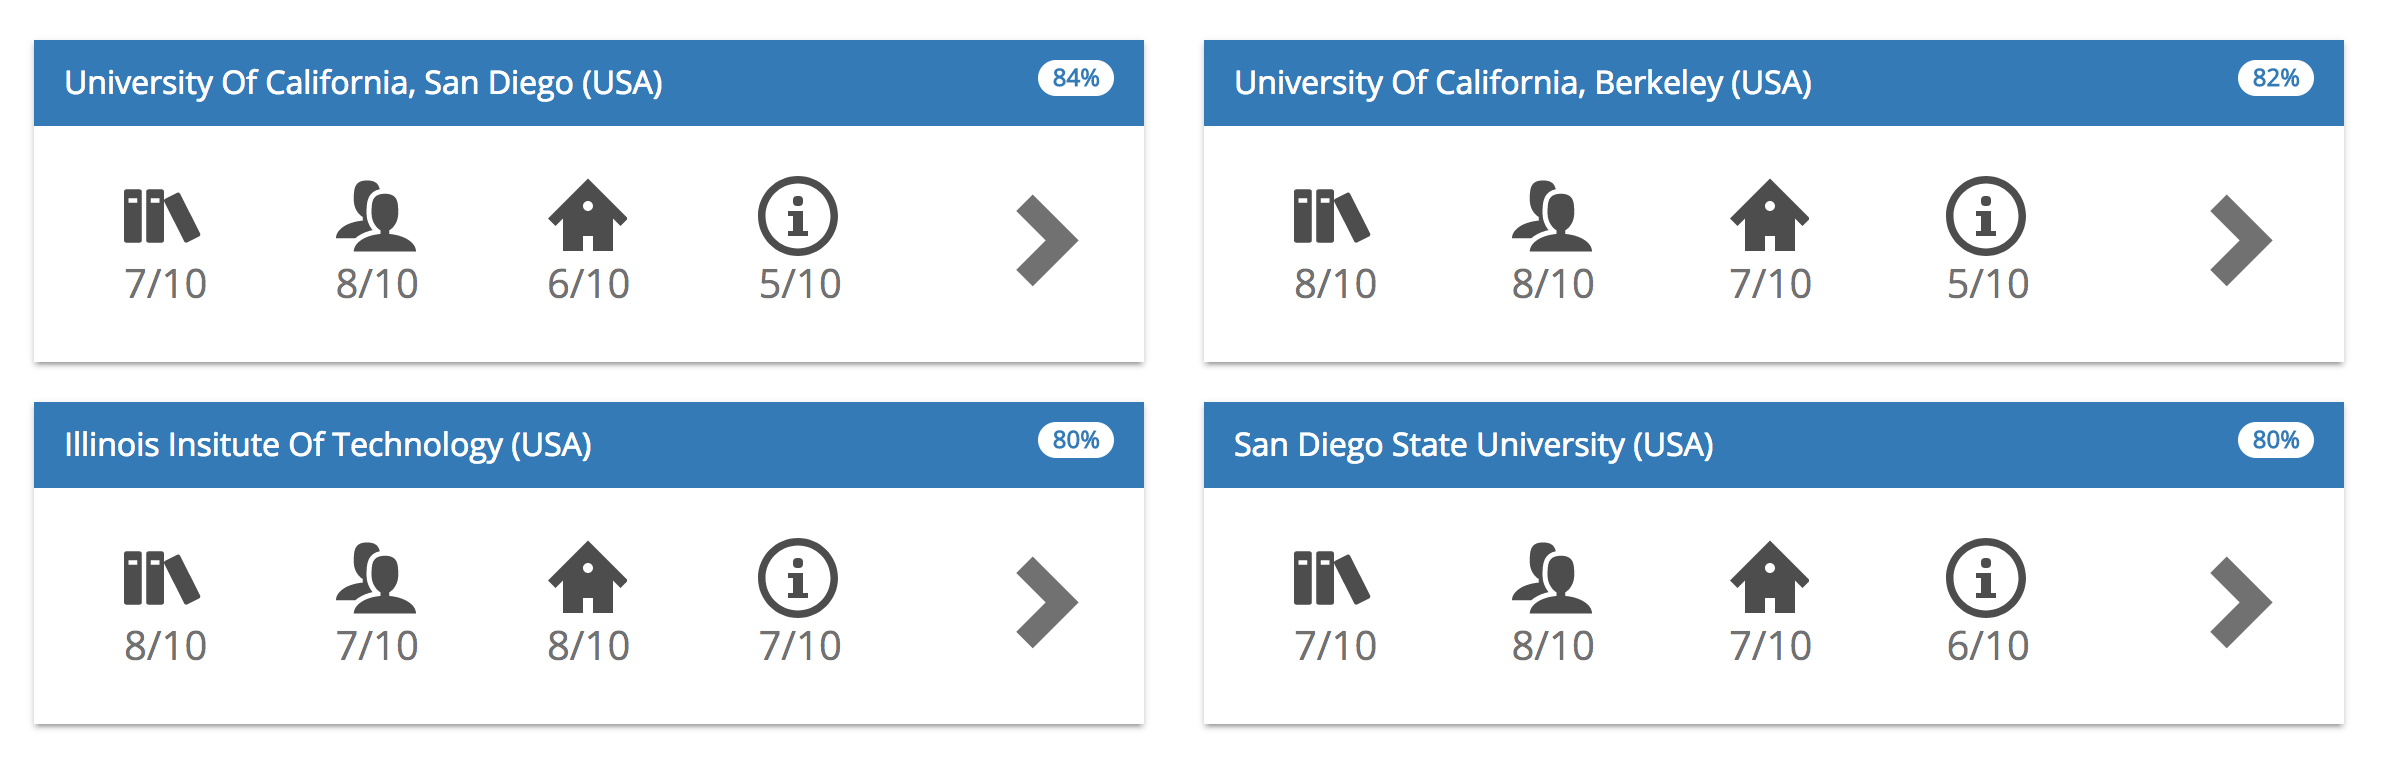
\includegraphics[width=1\textwidth]{fig/utsida_screenshots/result_1_cut_high.png}
    \caption{Recommendation view}
    \label{fig:web_results_1}
\end{figure}

\begin{figure}[h]
    \centering
    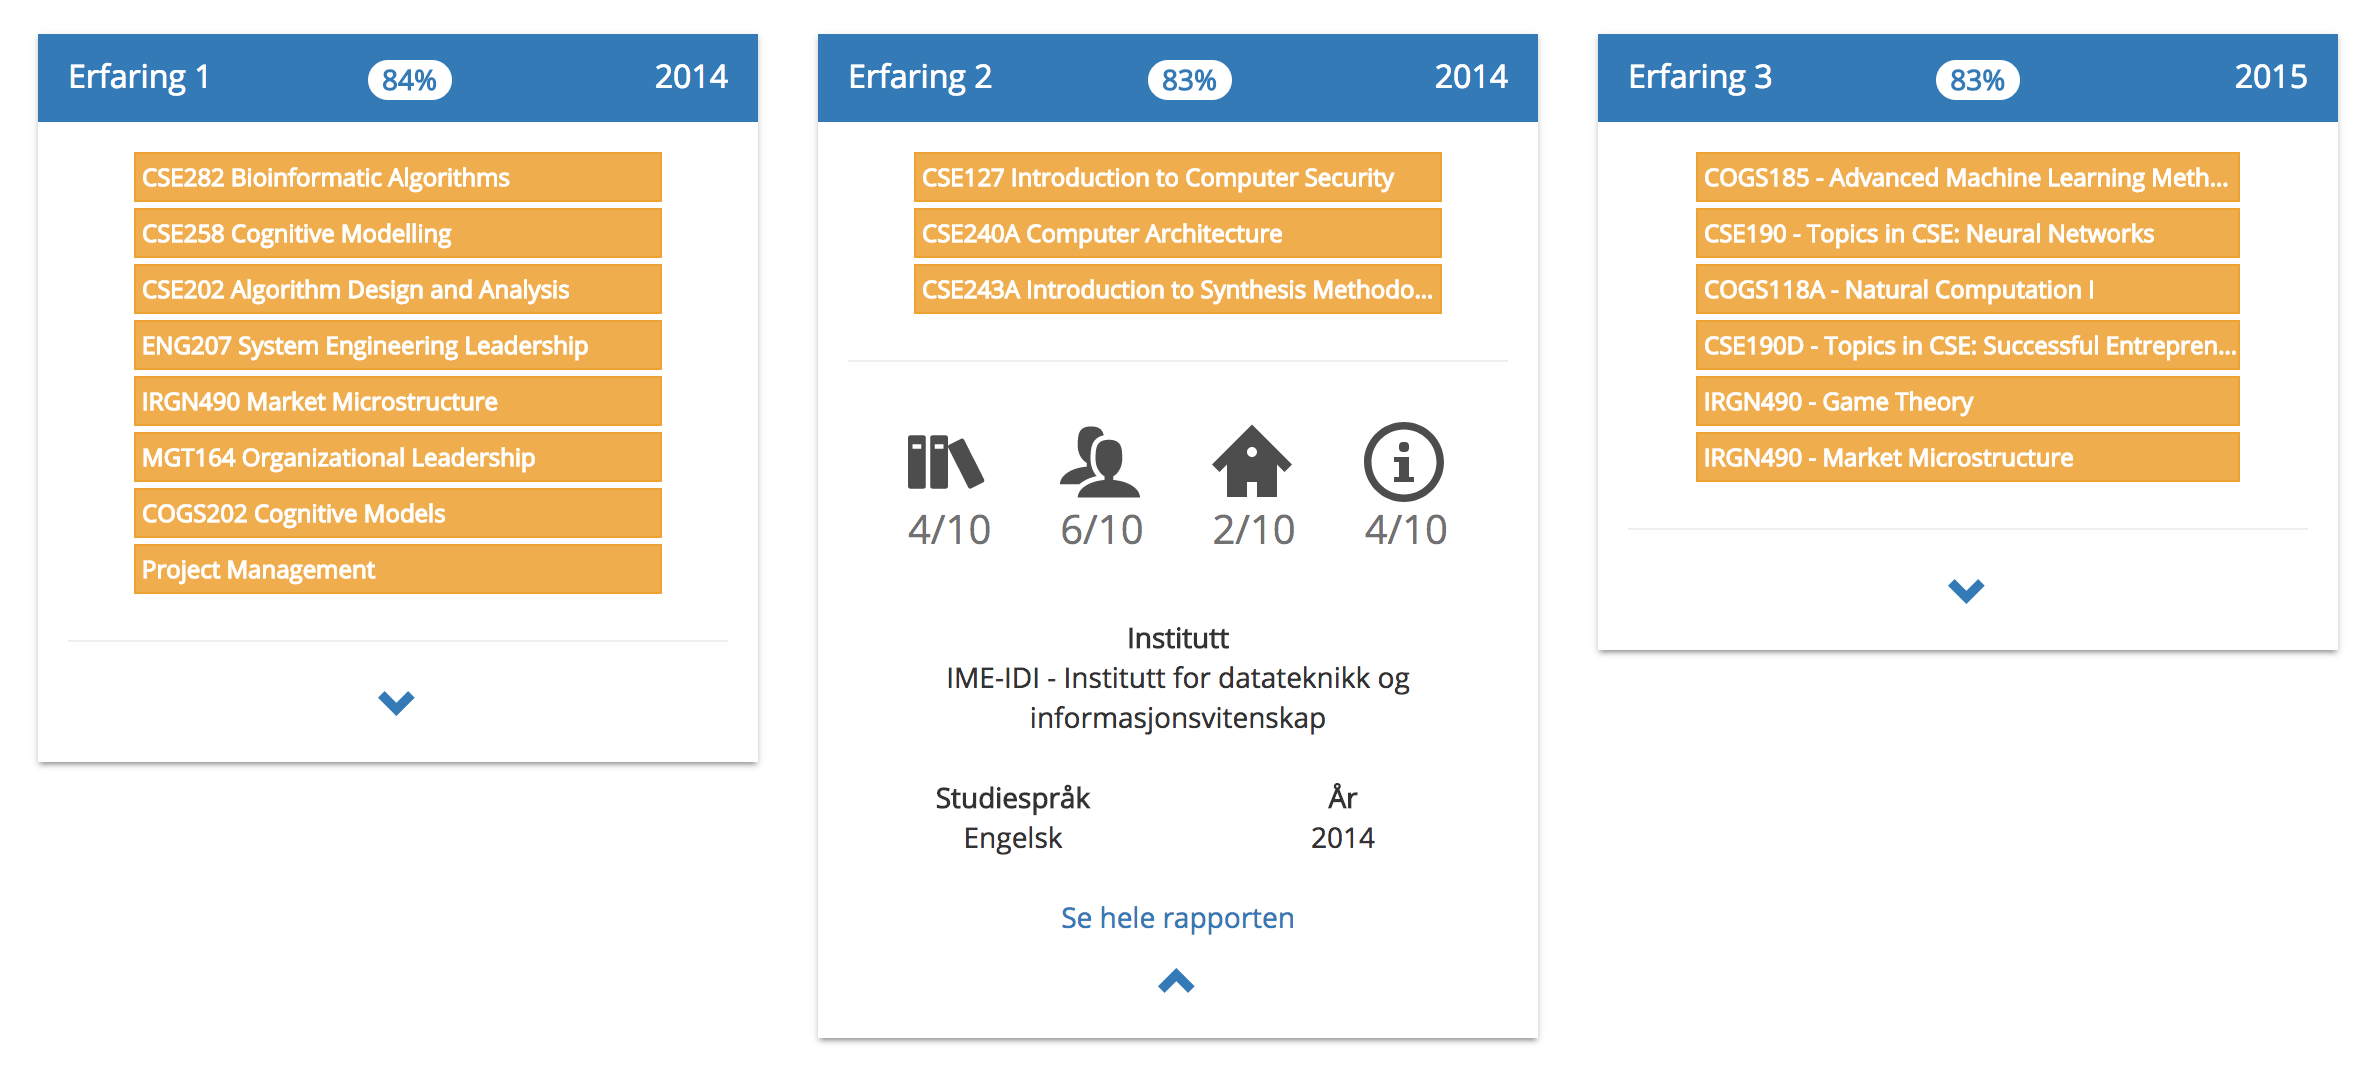
\includegraphics[width=1\textwidth]{fig/utsida_screenshots/result_2_cut_high.png}
    \caption[Course recommendation view]{Course recommendation view after selecting university}
    \label{fig:web_results_2}
\end{figure}

\begin{figure}[H]
    \centering
    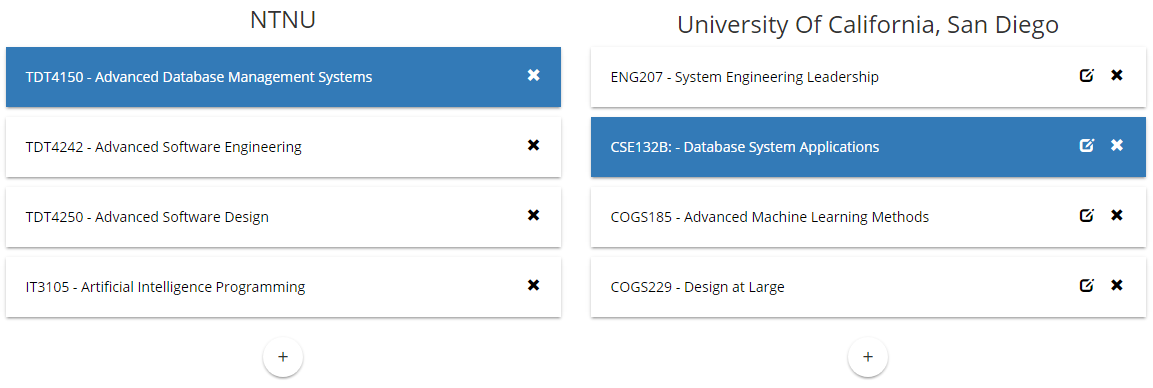
\includegraphics[width=1\textwidth]{fig/utsida_screenshots/course_match_cut.png}
    \caption{View for saving, viewing and matching courses}
    \label{fig:web_courses}
\end{figure}

\subsection{Tools and Frameworks}

When developing the web application part of Utsida, several tools and packages were used to simplify the development process and to implement functionality that was not feasible to develop from scratch.

To enforce a responsive and aesthetic design, Bootstrap 3\footnote{http://getbootstrap.com/} was used as the front-end Cascading Style Sheets (CSS) framework. jQuery\footnote{https://jquery.com/} was used to simplify HTTP requests, which this system largely relies on both internally in the web application and between the web application and the CBR-RS. A collection of packages for the Python language was also used. These packages include Fuzzywuzzy\footnote{https://pypi.python.org/pypi/fuzzywuzzy}: a packages which handles apprximate string matching, Requests\footnote{http://docs.python-requests.org/en/master/}: a package for writing HTTP requests from Python, and Python-social-auth\footnote{https://python-social-auth.readthedocs.io/en/latest/} combined with Dataporten-auth\footnote{https://pypi.python.org/pypi/dataporten-auth/0.1} to enable the use of authentication methods such as Feide, the authentication service used at NTNU.

Django\footnote{https://docs.djangoproject.com/en/1.11/}, a web framework using the Python programming language, was chosen as the web framework to use in the web application. Django is maintained by the Django Software Foundation (DSF). The DSF calls it an MTV-framework, meaning \emph{Model, Template, View}, which in practice functions as a Model View Controller (MVC) pattern. Django includes many built-in features: an SQLite database, a predefined directory structure, controllers to handle communication between the different components, and many others. Another important feature is Django's built-in security packages, which handles security risks such as Cross-Site Request Forgery, authorization, and Cross-Site Scripting. Django also includes an administrator panel, which enables management of database models with a simple interface. In conclusion, the reason for choosing Django as the main framework was because it offered a complete package that reduced the time used on structural difficulties and made it possible to focus on the usability and evaluation methods.

\subsection{Design Choices}
The design in terms of both functionality and aesthetics was an integral part of the development of the web application part of Utsida. Both of the questionnaires in the project were conducted remotely and were self-administered, which removes the option to help the participants with possible issues. Therefore, Utsida had to be designed in a way which would produce as little issues and hardships for the users as possible.

The design process of Utsida is inspired by the User Centered Design process, introduced by Norman and Draper \cite{norman1986user}. Potential users of the system were included throughout the development process, either with small interviews or larger usability tests. The results of these tests resulted in several identified problem areas. Measures were implemented to reduce the problem areas and strive for a user-centered design. Some of these measures were:

\begin{itemize}
    \item Personalized items: Buttons and links to parts of the application that contain user specific data are prefixed with the word "\emph{My}", for example: \emph{My courses, My profile, My applications}.
    \item Inline help text: Some parts of the application contain help text for users that may need it. The help texts are shown by hovering or clicking on a question mark button. 
    \item Streamlined process: The typical chronological use of Utsida is displayed as a numerated process to guide the user, as shown in Figure \ref{fig:utsida_index}.
\end{itemize}

\begin{figure}[h]
    \centering
    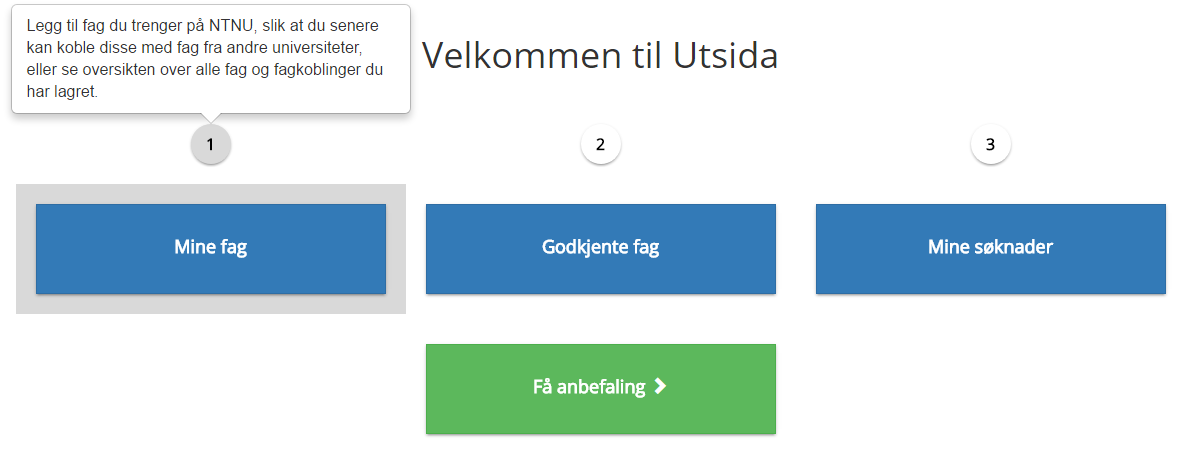
\includegraphics[width=1\textwidth]{fig/utsida_screenshots/steps.png}
    \caption[Home page of Utsida]{Home page of Utsida. Showing the process flow help text.}
    \label{fig:utsida_index}
\end{figure}

\section{The CBR-RS}

This section describes how the CBR-RS was modeled with myCBR Workbench and how it was implemented to give the most relevant recommendations. Furthermore, this section includes details on the case representation, the similarity measures used, how the weighting of the attributes in the exchange experience concept was done, and how the system itself is structured.

\subsection{Overview}

The CBR-RS is a customized version of an open-source Java Spring\footnote{https://spring.io/} application that implements the myCBR SDK. To serve requests from a web application, the Java application uses a REST API implemented with the Swagger API\footnote{http://swagger.io/}. This architecture made it possible to let the web application and the CBR-RS be two independent systems, only communicating through HTTP requests. The CBR-RS imports a custom myCBR project file which contains the exchange experience concept's case representation, the similarity measures used for each attribute and the attributes' weight values. It also imports a CSV file containing all the cases, used as the case-base.

When a request is made by a user in the web application, a query is first sent to the CBR-RS. When the CBR-RS receives the query, it performs the first step of the CBR-cycle by using the retrieve operation in the myCBR SDK. The myCBR SDK then returns the exchange experiences (i.e. cases) with their respective similarity scores. The exchange experiences are further ordered from highest to lowest similarity, and finally, the exchange experiences with the highest similarity scores are returned to the web application. Figure \ref{fig:retrieval_process_diagram} displays how a request made by a user in the web application traverse between the two systems to return a list of the most similar exchange experiences.

\begin{figure}[h]
    \centering
    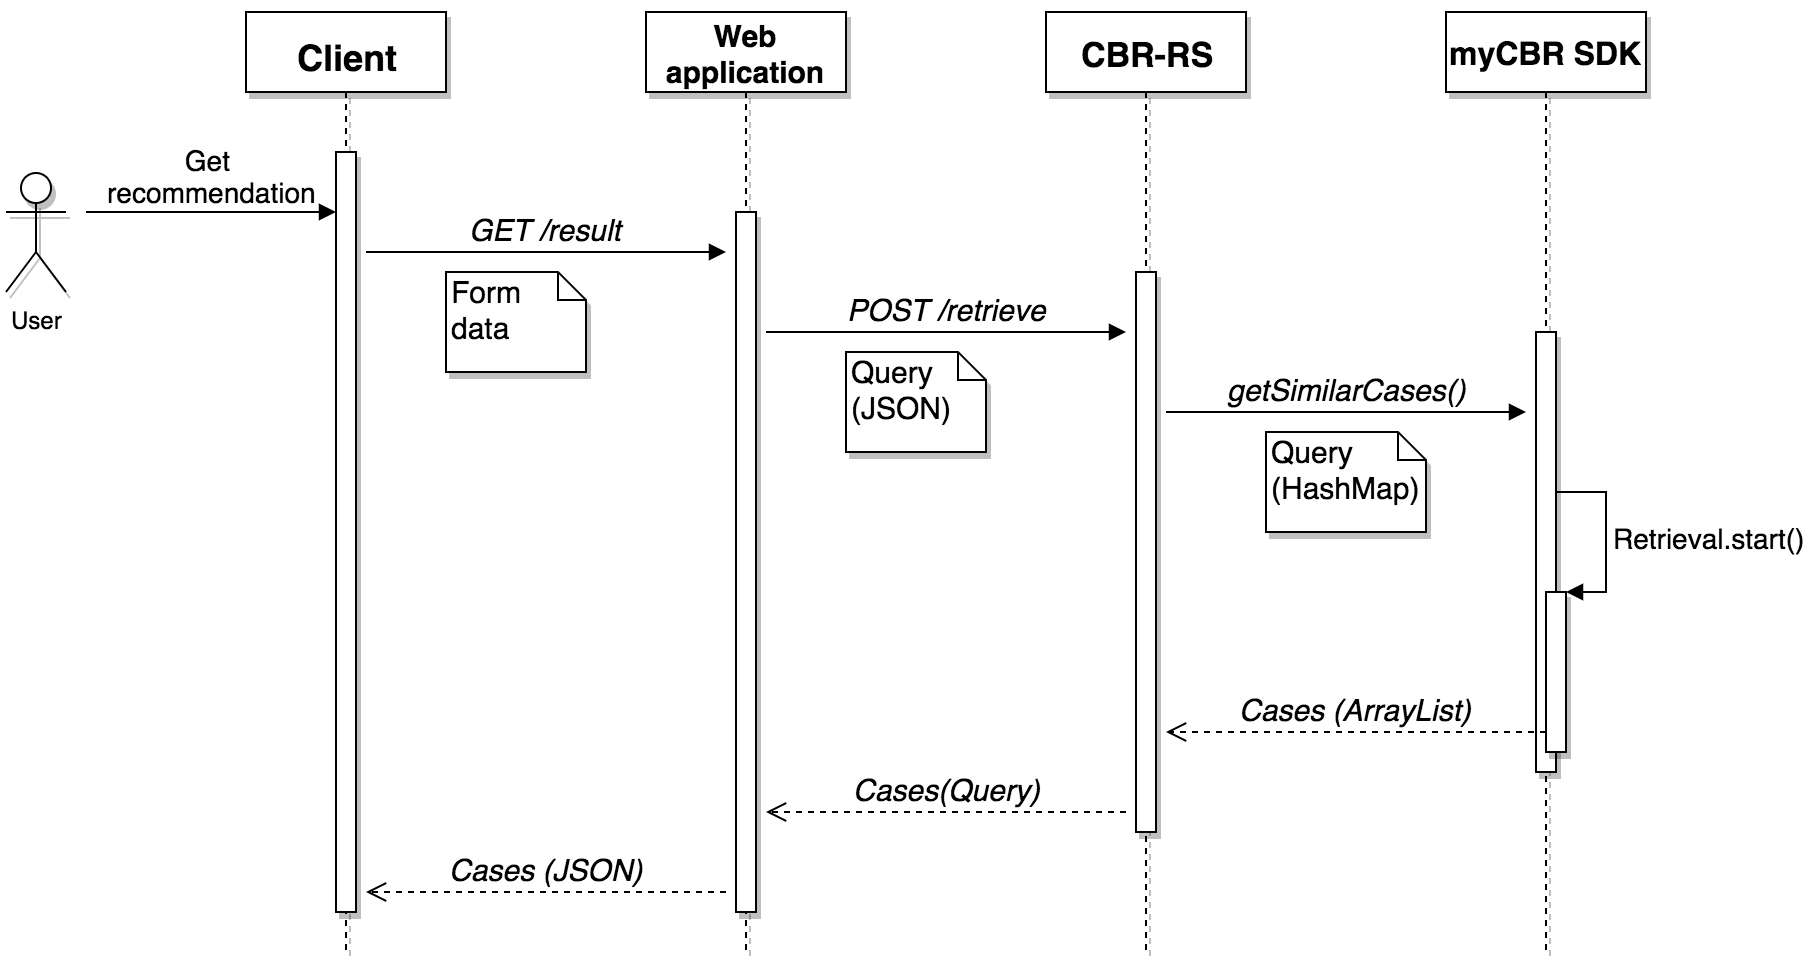
\includegraphics[width=1\textwidth]{fig/RetrievalProcessDiagram.png}
    \caption{Sequence diagram for a recommendation request in Utsida}
    \label{fig:retrieval_process_diagram}
\end{figure}

\subsection{Case Representation}

The exchange experience reports are the underlying data the CBR-RS use to give recommendations. These reports contain a significant amount of information and not all of it is relevant. Only a small part of the data was used to ensure that Utsida gives relevant recommendations and is straightforward to use. The first choice of information to use for the initial case representation were based on personal experiences and a study by Cubillo et. al. \cite{maria2006international} that identified groups of important motivational factors. This representation was, however, extended in an iterative process of usability tests and then finalized by using the results of questionnaire 1 (sec. \ref{sec:questionnaire_1}). The final case representation is displayed in Table \ref{tab:case_representation2}.

\begin{table}[h]
\centering
\small
\caption{Case representation in the CBR-RS}
\label{tab:case_representation2}
\begin{tabulary}{\textwidth}{|L|L|}
\hline
\textbf{Attributes} & \textbf{Example case values} \\ \hline \hline
Department & IME-IDI - Institutt for datateknikk og informasjonsvitenskap \\ \hline
Continent & North America \\ \hline
Country & USA \\ \hline
University & UCLA \\ \hline
Language & English \\ \hline
Study Period & 2012 \\ \hline
Academic Quality Rating & 8 \\ \hline
Social Quality Rating & 4 \\ \hline
Ease to find- and quality of residential & 5 \\ \hline
Support and reception at university & 6 \\ \hline
Subjects Taken & \begin{tabular}[c]{@{}l@{}}COMP1927 - Computing 2\\ MATH3220\\ CS4210\\ DATA101\end{tabular} \\ \hline
\end{tabulary}
\end{table}


\subsubsection{The Problem Part}

The problem part of a case is all attributes which denote a user's preferences for a query and profile information about them. The following list elaborate on the different attributes used in a case.

\begin{itemize}
\item \textbf{Department:} A profile attribute which details the department a user belongs to. It is considered the most important attribute, as it highly indicates what kind of courses (i.e. solution) that are relevant to a user. 

\item \textbf{Continent:} A preference attribute that implies what continent a user wish to travel to. Allows for a less precise location than a country.

\item \textbf{Country:} A preference attribute that implies what country a user wish to travel to. Serves as the most precise geographical location a user can select.

\item \textbf{University:} A preference attribute that lets a user include a specific university they wish to go to.

\item \textbf{Language:} A preference attribute that represents the language the user wish to study in.

\item \textbf{Study Period:} A hidden attribute that is the current year for a problem. In a case it is the year an exchange experience was written. The attribute is included to make older cases less relevant to the user, as university courses often change over time.

\item \textbf{Academic Quality Rating:} A preference attribute that is a conjunction of an experience report's \emph{Academic Quality}, \emph{Special Competence Gained} and general \emph{Quality of Academic Opportunities}. Each of these aspects is related to the academic quality of an experience, and are weighted differently.

\item \textbf{Social Quality Rating:} A preference attribute that is a conjunction of an experience report's rating of  \emph{Social Quality}, \emph{Leisure Activities}, \emph{Girlfriend/friends}, the social interaction with \emph{Students from the University}, \emph{Other Foreign Students} and \emph{Norwegian Students}. Each of these aspects is related to the social quality of an experience, and are weighted differently.

\item \textbf{Ease to find- and Quality of Residential:} A preference attribute that is a conjunction of an experience report's rating of \emph{Residential Dissemination} and \emph{Residential Quality}. Each of these aspects is related to the residential part of an experience, and are weighted differently.

\item \textbf{Support and Reception at University:} A preference attribute that is a conjunction of an experience report's rating of \emph{General Reception} and \emph{Administrative Support}. Each of these aspects is related to the support a student received at the university in an experience, and are weighted differently.
\end{itemize}

\subsubsection{The Solution Part}
The solution to a query is given by the set of courses in similar experiences. The university is however also a part of the recommendation and is used to filter the experiences, and can, therefore, be viewed as part of the solution.

\subsection{Similarity Measures}
Each attribute in the exchange experience concept was assigned a designated similarity measure. These measures returns a similarity score based on the similarity between the attribute in a query and the coherent attribute in a case. Following, each of the used measures are detailed and explained.


\subsubsection{Rating Similarity} 

In the exchange experience concept, the attributes \emph{AcademicQuality}, \emph{SocialQuality}, \emph{ReceptionQuality} and \emph{ResidentialQuality} are conjunctions of different ratings in the experience reports. Each rating ranges between 1-10 and reflects how the student experienced these categories. To calculate the similarity between a rating in a case, and a rating from a query, the CBR-RS uses Symmetric Difference Determined Similarity \cite{bergmann2002experience} with a linear function (equation \ref{eq:rating_sim}). It describes the decrease in similarity at a linear rate.


\begin{equation} \label{eq:rating_sim}
    f(d) = 
    \begin{cases} 1 : & d < min \\ 
    \frac{max-d}{max-min} : & min \leq d \leq max \\
    0 : & d > max
    \end{cases}
\end{equation}


\subsubsection{Continent Similarity} 

The continent attribute is a \textit{symbol} type, meaning its allowed values are a pre-determined set. The similarity between continents is calculated with an $m \, x \, n$-matrix, where each mapping between two different continents yields a given similarity, as displayed in Table \ref{tab:continent_similarity}. The values were chosen to represent similarity in culture, language, location, and general university structure.

\begin{table}[H]
\small
\centering
\caption{Matrix for calculating similarity between continents}
\label{tab:continent_similarity}
\begin{tabular}{|
>{\columncolor[HTML]{C0C0C0}}l |
>{\columncolor[HTML]{FFFFFF}}r |
>{\columncolor[HTML]{FFFFFF}}r |
>{\columncolor[HTML]{FFFFFF}}r |
>{\columncolor[HTML]{FFFFFF}}r |
>{\columncolor[HTML]{FFFFFF}}r |
>{\columncolor[HTML]{FFFFFF}}r |}
\hline
Attribute value & \cellcolor[HTML]{C0C0C0}South America & \cellcolor[HTML]{C0C0C0}Asia & \cellcolor[HTML]{C0C0C0}Europe & \cellcolor[HTML]{C0C0C0}Africa & \cellcolor[HTML]{C0C0C0}North America & \cellcolor[HTML]{C0C0C0}Oceania \\ \hline 
South America & 1.0 & 0.0 & 0.2 & 0.0 & 0.3 & 0.0 \\ \hline
Asia & 0.0 & 1.0 & 0.0 & 0.0 & 0.0 & 0.0 \\ \hline
Europe & 0.2 & 0.0 & 1.0 & 0.0 & 0.2 & 0.2 \\ \hline
Africa & 0.0 & 0.0 & 0.0 & 1.0 & 0.0 & 0.0 \\ \hline
North America & 0.3 & 0.0 & 0.2 & 0.0 & 1.0 & 0.2 \\ \hline
Oceania & 0.0 & 0.0.0 & 0.2 & 0.0 & 0.2 & 1.0 \\ \hline
\end{tabular}
\end{table}
    
\subsubsection{Country and Department Similarity} 
The Country- and Department attributes are structured as a taxonomy. A taxonomy can be used as a type of similarity measure \cite{richter2013case} and gives a similarity between similar groups of objects. For the country attribute, the taxonomy gives a similarity if the country resides within the same continent (i.e. group) as the country in the query. If the countries in the query and a case are the same, the similarity score will be 1.0. If the countries are different, but still resides within the same continent, the similarity score will be set according to Table \ref{tab:taxonomic_continent_similarity}. The same taxonomy is also in place for the Department attribute, however, the departments are instead grouped by faculty. The similarity score between departments in the same faculty is set to 0.3.

\begin{table}[h]
\centering
\caption{Taxonomic similarity of each continent}
\label{tab:taxonomic_continent_similarity}
\begin{tabulary}{\textwidth}{|L|L|}
\hline
\textbf{Continent} & \textbf{Similarity} \\ \hline \hline
North America & 0.2 \\ \hline
South America & 0.3 \\ \hline
Oceania & 0.4 \\ \hline
Asia & 0.3 \\ \hline
Europe & 0.2 \\ \hline
Africa & 0.4 \\ \hline
\end{tabulary}
\end{table}
    
\subsubsection{Language Similarity} 

The language attribute is represented as a symbol type, which allows the attribute to contain multiple languages. If a case contains more than one language, the similarity measure will return the mean similarity to all languages in that case. If a case only contains one language, it will either return a similarity score of 1.0 (if the language in the query and case are is the same), or else 0.0. For example, if a query contains the language \textit{Spanish} and a case contains the languages \textit{English, Spanish, Portuguese}, the similarity score will be 0.33.
    
\subsubsection{University Similarity} 

The university attribute is a string type. The similarity measure between two universities returns 1.0 if they are a complete match, or 0.0 if they differ in any way. It would be desirable to have partial similarity for two strings, but this functionality is not included in myCBR.
    
\subsubsection{Study Period Similarity} 

The similarity measure used for the study period attribute is defined by a declining graph, where the similarity score decrease according to the distance in years between the query and a case. The similarity greatly decreases until a case is 9 years old. Figure \ref{fig:study_period_graph} illustrates the graph.
    
\begin{figure}[h]
    \centering
    \caption[Study period similarity measure]{Study period similarity measure given by the distance in years between a query and a case.}
    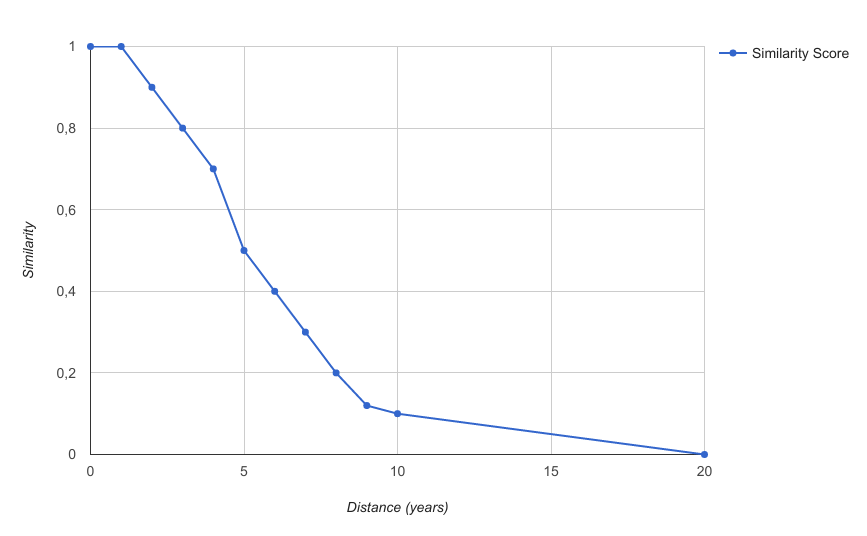
\includegraphics[width=1.0\textwidth]{fig/study_period_graph.png}
    \label{fig:study_period_graph}
\end{figure}

\subsection{Summation Function}

Multi-Criteria Decision Making Methods (MCDMM) are used in myCBR as summation functions that combine the similarity score of each attribute in the concept, with regards to the attribute's weight. The myCBR Workbench has two MCDMMs, the Weighted Sum Model (WSM) and the Euclidean Distance. For single dimensional problems, which are the types of problems in the CBR-RS, the WSM can be used without difficulties, and is probably the most common approach \cite{triantaphyllou2000multi} (equation \ref{eq:WSM} \cite{fishburn1967letter}).

\begin{equation} \label{eq:WSM}
    A^{*}_{WSM-score}\quad =\quad max_{i}\  \sum\limits_{j = 1}^{n}\  a_{ij}w_{j},\quad for \quad i =1,\ 2,\ 3,\ ...,\ m.
\end{equation}

When the CBR-RS receives a query, a decision matrix is calculated for each case. This is an $(m \times n)$ matrix where each row contains the attribute values and weight of a case, as shown in Table \ref{tab:decision_matrix}. The WSM is used on this matrix to give each case in the case-base a similarity score between 0.0-1.0.


\begin{table}[h]
\centering
\caption[Decision matrix for a query]{Decision matrix example for calculating similarity between a query and the cases in the case-base}
\label{tab:decision_matrix}
\begin{tabular}{ccccccc}
\cline{2-7}
\multicolumn{1}{l|}{} & \multicolumn{1}{c|}{\textbf{Attribute}} & \multicolumn{1}{c|}{Country} & \multicolumn{1}{c|}{Language} & \multicolumn{1}{c|}{\ldots} & \multicolumn{1}{c|}{\ldots} & \multicolumn{1}{c|}{AcademicQuality} \\ \cline{2-7} 
\multicolumn{1}{l|}{} & \multicolumn{1}{c|}{\textbf{Weight}} & \multicolumn{1}{c|}{$w_{country}$} & \multicolumn{1}{c|}{$w_{language}$} & \multicolumn{1}{c|}{\ldots} & \multicolumn{1}{c|}{\ldots} & \multicolumn{1}{c|}{$w_{country}$} \\
\hline
\multicolumn{1}{|c|}{\multirow{5}{*}{\textbf{Cases}}} & \multicolumn{1}{c|}{$case_{1}$} & \multicolumn{1}{c|}{$sim_{case_{1}}$} & \multicolumn{1}{c|}{$sim_{case_{1}}$} & \multicolumn{1}{c|}{\ldots} & \multicolumn{1}{c|}{\ldots} & \multicolumn{1}{c|}{$sim_{case_{1}}$} \\
\multicolumn{1}{|c|}{} & \multicolumn{1}{c|}{$case_{2}$} & \multicolumn{1}{c|}{$sim_{case_{2}}$} & \multicolumn{1}{c|}{$sim_{case_{2}}$} & \multicolumn{1}{c|}{\ldots} & \multicolumn{1}{c|}{\ldots} & \multicolumn{1}{c|}{$sim_{case_{2}}$} \\
\multicolumn{1}{|c|}{} & \multicolumn{1}{c|}{.} & \multicolumn{1}{c|}{.} & \multicolumn{1}{c|}{.} & \multicolumn{1}{c|}{\ldots} & \multicolumn{1}{c|}{\ldots} & \multicolumn{1}{c|}{.} \\
\multicolumn{1}{|c|}{} & \multicolumn{1}{c|}{.} & \multicolumn{1}{c|}{.} & \multicolumn{1}{c|}{.} & \multicolumn{1}{c|}{\ldots} & \multicolumn{1}{c|}{\ldots} & \multicolumn{1}{c|}{.} \\
\multicolumn{1}{|c|}{} & \multicolumn{1}{c|}{$case_{m}$} & \multicolumn{1}{c|}{$sim_{case_{m}}$} & \multicolumn{1}{c|}{$sim_{case_{m}}$} & \multicolumn{1}{c|}{\ldots} & \multicolumn{1}{c|}{\ldots} & \multicolumn{1}{c|}{$sim_{case_{m}}$} \\ \hline
\multicolumn{1}{l}{} & \multicolumn{1}{l}{} & \multicolumn{1}{l}{} & \multicolumn{1}{l}{} & \multicolumn{1}{l}{} & \multicolumn{1}{l}{} & \multicolumn{1}{l}{}
\end{tabular}
\end{table}


\subsection{Attribute Weights}\label{sec:weighting}

Each attribute in a concept has a value and an associated weight. This is essentially an integer denoting the importance of that attribute. The results of questionnaire 1 (Table \ref{tab:attribute_ranking}), were used to decide the final weight of the different attributes in the exchange experience concept, shown in Table \ref{tab:attribute_weights}.

\begin{table}[h]
\centering
\caption{Weighting of the concept's attributes}
\label{tab:attribute_weights}
\begin{tabulary}{\textwidth}{|L|R|}
\hline
\textbf{Attribute} & \textbf{Weight} \\ \hline \hline
Department & 7.0 \\ \hline
Continent & 2.5 \\ \hline
Country & 4.0 \\ \hline
University & 4.0 \\ \hline
Language & 4.0 \\ \hline
Study period & 4.5 \\ \hline
Academic Quality Rating & 3.0 \\ \hline
Social Quality Rating & 3.0 \\ \hline
Ease to find- and quality of residential & 1.5 \\ \hline
Support and reception at university & 2.5 \\ \hline
\end{tabulary}
\end{table}

\FloatBarrier
\section{Test Environment}
The test environment used by Utsida is an essential part of the project because it was the platform used for the user study in questionnaire 2. Utsida was hosted on a Ubuntu 16.04\footnote{Ubuntu, a Debian-based Linux operating system. https://www.ubuntu.com/} virtual server provided by IDI with the domain name utsida.idi.ntnu.no. The specific HTTP web server used was Apache2\footnote{https://httpd.apache.org/}, and it was configured with HTTPS to enable secure and encrypted user sessions. Support for registering and logging in with users university accounts was implemented to reduce the effort for users to participate in online usability tests and user study. The service platform "Dataporten"\footnote{https://www.uninett.no/en/dataporten} provided by UNINETT made it possible to use the university account registration through UNINETT's federated authentication service (FEIDE).

Error reporting through email was configured on the server so that alerts were given in case of possible downtime or server errors. Error reporting made it possible to quickly resolve potential bugs or errors on the application and ensure high user satisfaction during the user tests. Specific user behavior and statistics was tracked by using Google Analytics, this was useful in the final data to increase the understanding of user behaviors. By using Google Analytics it is possible to see a large set of data on the user behavior. The most important data used in this project were number of users, average session time, device type and activity flow.  

\cleardoublepage